\renewcommand{\captiontitle}{Orthogonal clinical views in canonical orientation}
\begin{figure*}
\begin{center}

\setlength{\tabcolsep}{1pt}

\begin{tabular}{ccccc}

\toprule
\SA{} (Base) & \SA{} (Midslice) & \SA{} (Apex) & \HLA{} & \VLA{} \\
\midrule

\multicolumn{5}{c}{Original Untransformed Image: $\image$} \\

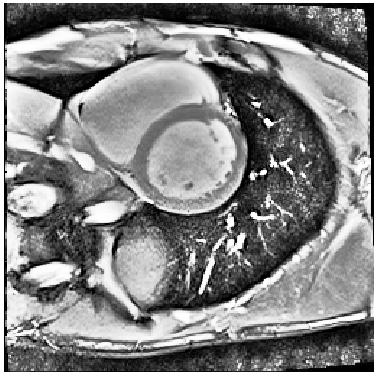
\includegraphics[width=0.19\textwidth]{./data/ohm/control/HCMNet_1100594/00_SAX/35_/im.png} &
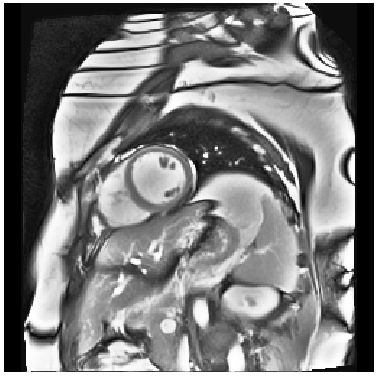
\includegraphics[width=0.19\textwidth]{./data/ohm/control/HCMNet_1100823/00_SAX/33_/im.png} &
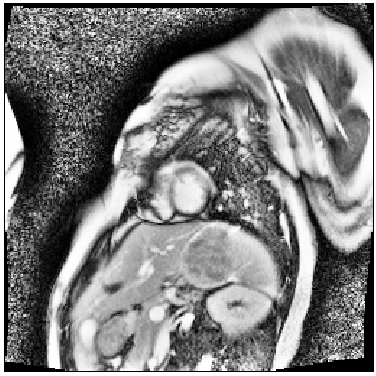
\includegraphics[width=0.19\textwidth]{./data/ohm/control/HCMNet_2600035/00_SAX/024_SA_CINE/im.png} &
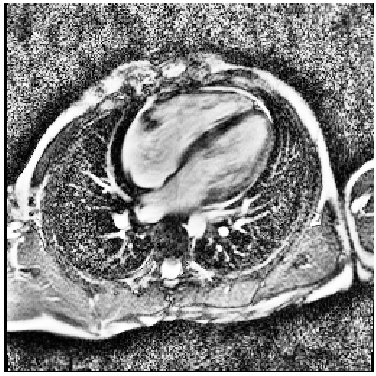
\includegraphics[width=0.19\textwidth]{./data/ohm/control/HCMNet_1700012/01_HLA/00/im.png} &
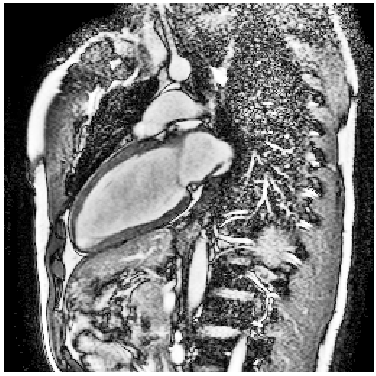
\includegraphics[width=0.19\textwidth]{./data/ohm/control/HCMNet_2100096/02_VLA/00/im.png} \\

\multicolumn{5}{c}{Structure \hl{Localization}} \\

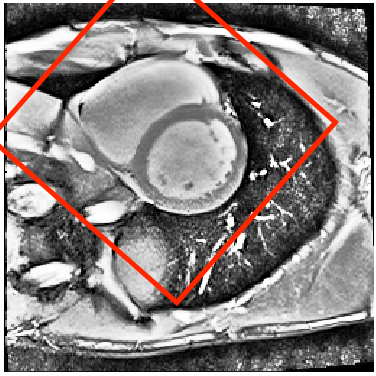
\includegraphics[width=0.19\textwidth]{./data/ohm/control/HCMNet_1100594/00_SAX/35_/im_det.png} &
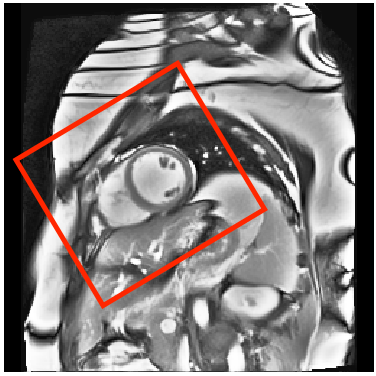
\includegraphics[width=0.19\textwidth]{./data/ohm/control/HCMNet_1100823/00_SAX/33_/im_det.png} &
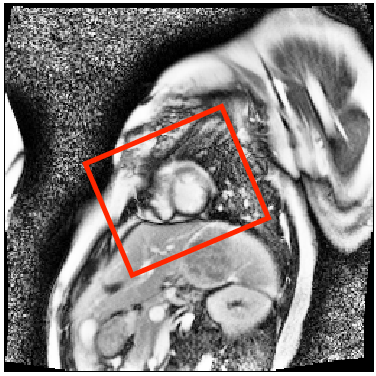
\includegraphics[width=0.19\textwidth]{./data/ohm/control/HCMNet_2600035/00_SAX/024_SA_CINE/im_det.png} &
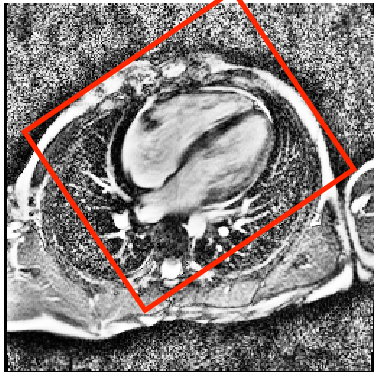
\includegraphics[width=0.19\textwidth]{./data/ohm/control/HCMNet_1700012/01_HLA/00/im_det.png} &
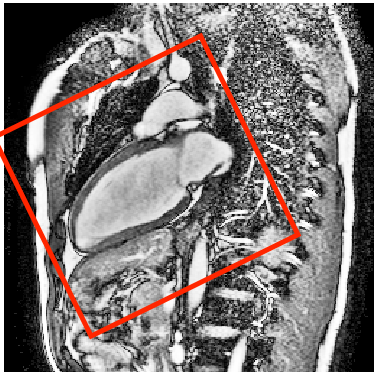
\includegraphics[width=0.19\textwidth]{./data/ohm/control/HCMNet_2100096/02_VLA/00/im_det.png} \\

\multicolumn{5}{c}{Image in Canonical Orientation: $\image^\prime = \trans(\image,M)$} \\

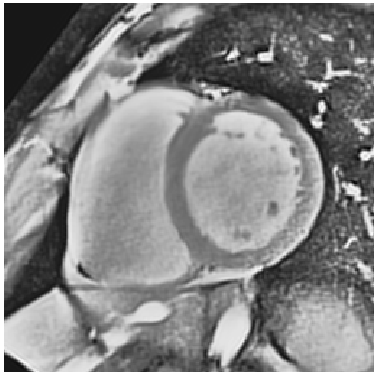
\includegraphics[width=0.19\textwidth]{./data/ohm/control/HCMNet_1100594/00_SAX/35_/im_t.png} &
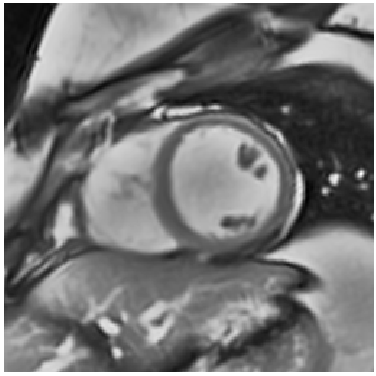
\includegraphics[width=0.19\textwidth]{./data/ohm/control/HCMNet_1100823/00_SAX/33_/im_t.png} &
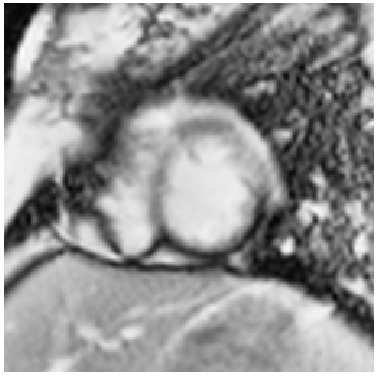
\includegraphics[width=0.19\textwidth]{./data/ohm/control/HCMNet_2600035/00_SAX/024_SA_CINE/im_t.png} &
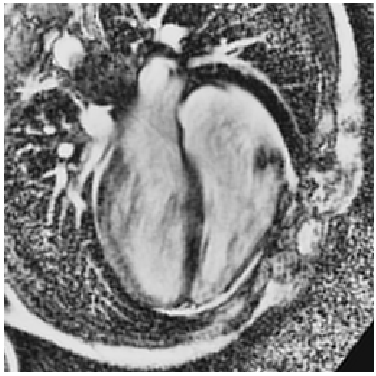
\includegraphics[width=0.19\textwidth]{./data/ohm/control/HCMNet_1700012/01_HLA/00/im_t.png} &
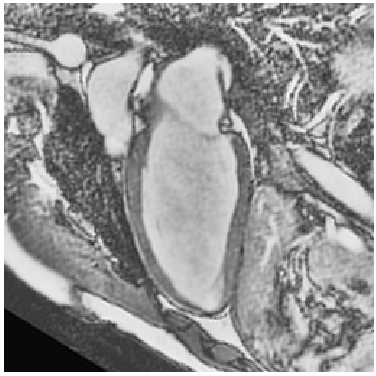
\includegraphics[width=0.19\textwidth]{./data/ohm/control/HCMNet_2100096/02_VLA/00/im_t.png} \\
\bottomrule

\end{tabular}

\caption[\captiontitle]{\captiontitle{}.
Representative short axis (\SA{}), four-chamber (\HLA{}), and two-chamber (\VLA{}) images are shown as acquired (top), and having undergone rigid, affine transformation into a canonical orientation (bottom).
Consistent with common clinical practice, the heart is rotated such that in the \SA{} views, the right ventricle appears on the (radiological) right side of the image, whereas in the \HLA{} and \VLA{} views, the long axis of the left ventricle is oriented vertically.
The heart is also centered and scaled to fill $90\%$ of the image.
Note the heterogeneity in size, orientation, and appearance of the heart in the untransformed images, which contributes to the difficulty of segmentation.
}
\label{fig:canonical-orientation}
\end{center}
\end{figure*}
